%%%%%%%%%%%%%%%%%%%%%%%%%%
%% Folie: PreProcessing %%
%%%%%%%%%%%%%%%%%%%%%%%%%%
\begin{frame}
    \frametitle{Pre-processing -- Data}
\vspace*{0.8cm}

\begin{multicols}{2}
    \textbf{Input channels}\newline
    \vspace*{0.6cm}
    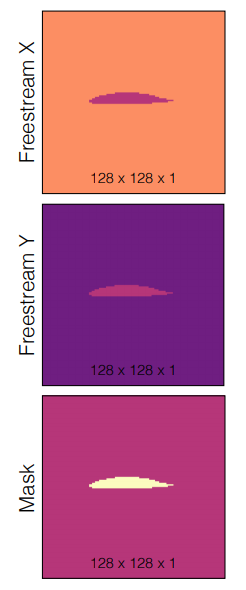
\includegraphics[width=0.15\textwidth, height=.45\textheight]{./Ressourcen/Praesentation/Bilder/sampleInput.png}

%1. Bit mask representing airfoil shape
  
%2. $x$ velocity component
   
%3. $y$ velocity component
\vspace*{-0.9cm}
Reynolds number encoded as differently scaled \newline freestream velocity vectors wrt. their magnitude
    \vfill\columnbreak
    \textbf{Target channels}\newline
    \vspace*{0.6cm}
    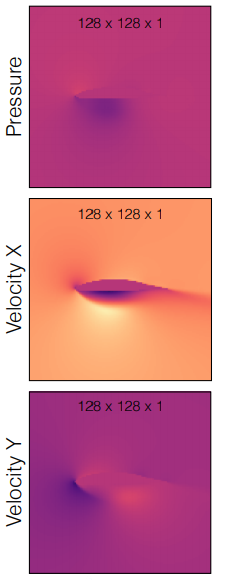
\includegraphics[width=0.15\textwidth, height=.45\textheight]{./Ressourcen/Praesentation/Bilder/sampleTarget.png}

%1. Pressure field
  
%2. $x$ velocity field
   
%3. $y$ velocity field
\vspace*{-0.9cm}
Data from the RANS solution
\end{multicols}

\end{frame}
\clearpage

\begin{frame}
    \frametitle{Pre-processing -- Normalization}
\vspace*{0.8cm}

Motivation: Flatten space of solutions, accelerate learning by simplifing the learning task for the NN

Normalization of target channels by division with freestream magnitude (vector norm, default: L2):\newline
This makes pressure and velocity dimensionless

$\tilde{v_{o}} = \frac{v_{o}}{\|v_{i}\|}, \quad \tilde{p_{o}} = \frac{p_{o}}{\|v_{i}\|^{2}}$ -- important to remove quadratic scaling of pressure

For a better understanding: \newline
Pressure: $[p]_{SI} = 1 Pa = 1 \frac{kg}{m \cdot s^2}$ \newline
Density: $[\rho]_{SI} = 1 \frac{kg}{m^3}$ -- constant in incompressible flow \newline
Velocity: $[v]_{SI} = \frac{m}{s}$ \newline

\end{frame}
\clearpage

\begin{frame}
    \frametitle{Pre-processing -- Offset removal \& value clamping}
\vspace*{0.8cm}
Motivation: eliminate ill-posed learning goal \& improve numerical precision

Spatially move pressure distribution into the origin -- RANS typically only needs $\nabla_{p}$ for computation

$\hat{p_o} = \tilde{p_o} - p_{mean}$    

Clamp both input and target channels into $[-1, 1]$ range by diving by the maximum absolute value

\end{frame}
\clearpage

%%%%%%%%%%%%%%%%%%%%%%%%%%%%%%%%%%%%%%%%%%%%%%%%%%%%%
%% Folie: Diagramm                                 %%
%%%%%%%%%%%%%%%%%%%%%%%%%%%%%%%%%%%%%%%%%%%%%%%%%%%%%
\begin{frame}
    \frametitle{Pre-processing -- Evaluation}
 Vector norms used in pre-processing comparision wrt. error, default: L2 (in \%)\newline
 L1 normalization achieves the best error rates (p, vel, combined: \textbf{14.19}\%, \textbf{2.251}\%, \textbf{2.646}\% -- L2: 14.76\%, 2.291\%, 2.780\%)\newline
\begin{center}
	\vspace*{-1.5cm}
    \begin{tikzpicture}
        \begin{axis}[
                ybar=10,
                bar width=22.5,
                axis line style={transparent},
                every tick/.style={transparent},
                enlarge x limits=0.145, % X-Achse skalieren
                clip limits=true,
                ymin=0,
                ymax=35,
                width=\textwidth,
                height=.65\textheight,
                symbolic x coords={L1,L2,L Infinity,L 0.25, L 0.5, L 0.75},
                xticklabels={L1,L2,L Infinity,L 0.25, L 0.5, L 0.75},
                xtick=data,
                ytick={0,5,10,15,20,25,30},
                %ytick={0,2.5,5,10,,20,30},
                every tick label/.append style={font=\fontsize{13}{14}\selectfont},
                ymajorgrids,
                legend image code/.code={\draw[draw=none] (0cm,-0.12cm) rectangle (0.29cm,0.17cm);}, % Legenden-Symbol  
                legend columns=3,
                reverse legend,
                legend style={
                    font={\usebeamerfont{footnote}},
                    fill=none,
                    draw=none,
                    /tikz/every odd column/.append style={column sep=0.07cm}, % Abstand zwischen Legenden-Symbol
                    /tikz/every even column/.append style={column sep=0.8cm} % Abstand zwischen den Legendeneinträgen
                 },
                legend to name=PraesentationDiagrammVertikalLegende
            ]
            
            \addlegendentry{Combined}        
            \addlegendentry{Pressure}    
            \addlegendentry{Velocity}    
            
            %comb
            \addplot[color=TUMBlauDunkel, fill=TUMBlauDunkel] coordinates {
                (L1,2.67)
                (L2,2.78)
                (L Infinity,2.86)
                (L 0.25,3.27)
                (L 0.5,2.7)
                (L 0.75,3.27)
            };
            
            %p
            \addplot[color=TUMBlauHell, fill=TUMBlauHell] coordinates {
                (L1,14.19)
                (L2,14.76)
                (L Infinity,15.09)
                (L 0.25,31.03)
                (L 0.5,15.64)
                (L 0.75,31.03)
            };
            
            %v
            \addplot[color=TUMBlauMittel, fill=TUMBlauMittel] coordinates {
                (L1,2.25)
                (L2,2.29)
                (L Infinity,2.34)
                (L 0.25,3.1)
                (L 0.5,2.44)
                (L 0.75,3.1)
            };        
        \end{axis}
    \end{tikzpicture}

    \vspace*{-8mm}
    \ref*{PraesentationDiagrammVertikalLegende}%
\end{center}
\end{frame}
\clearpage